\documentclass{article}


% if you need to pass options to natbib, use, e.g.:
%     \PassOptionsToPackage{numbers, compress}{natbib}
% before loading neurips_2022


% ready for submission
% \usepackage{neurips_2022}


% to compile a preprint version, e.g., for submission to arXiv, add add the
% [preprint] option:
% \usepackage[preprint]{neurips_2022}


% to compile a camera-ready version, add the [final] option, e.g.:
  \usepackage[final]{neurips_2022}


% to avoid loading the natbib package, add option nonatbib:
%  \usepackage[nonatbib]{neurips_2022}


\usepackage[utf8]{inputenc} % allow utf-8 input
\usepackage[T1]{fontenc}    % use 8-bit T1 fonts
\usepackage{hyperref}       % hyperlinks
\usepackage{url}            % simple URL typesetting
\usepackage{booktabs}       % professional-quality tables
\usepackage{amsfonts}       % blackboard math symbols
\usepackage{nicefrac}       % compact symbols for 1/2, etc.
\usepackage{microtype}      % microtypography
\usepackage{xcolor}         % colors
\usepackage{graphicx}
\usepackage{subcaption}
\usepackage{caption}

\usepackage{fancyhdr}
\usepackage{extramarks}
\usepackage{amsmath}
\usepackage{amsthm}
\usepackage{amsfonts}
\usepackage{tikz}

\title{Tridimensional Regularization with Analysis in Social Network for Recommender Systems}


% The \author macro works with any number of authors. There are two commands
% used to separate the names and addresses of multiple authors: \And and \AND.
%
% Using \And between authors leaves it to LaTeX to determine where to break the
% lines. Using \AND forces a line break at that point. So, if LaTeX puts 3 of 4
% authors names on the first line, and the last on the second line, try using
% \AND instead of \And before the third author name.


\author{
  Chaofan Lin \\
    520021911042\\
    ACM Class 2020\\
    Zhiyuan College, Shanghai Jiao Tong University \\
  \texttt{siriusneo@sjtu.edu.cn} \\
  % examples of more authors
  % \And
  % Coauthor \\
  % Affiliation \\
  % Address \\
  % \texttt{email} \\
  % \AND
  % Coauthor \\
  % Affiliation \\
  % Address \\
  % \texttt{email} \\
  % \And
  % Coauthor \\
  % Affiliation \\
  % Address \\
  % \texttt{email} \\
  % \And
  % Coauthor \\
  % Affiliation \\
  % Address \\
  % \texttt{email} \\
}


\begin{document}


\maketitle

\begin{abstract}
  Matrix factorization with social regularization is a simple but effective social 
  recommending approach. However, there is still 
  much information in social networks
  waiting for us to extract.
  In this paper, we try to improve this model 
  by weighing friends with similarity, influence and familiarity.
  We perform empirical studies 
  on three different datasets to compare their effectiveness.
\end{abstract}


\section{Introduction}

Recommender systems have become a hot research topic recently
due to its commercial value and its role in satisfying users'
need of information. By the fact that the dimension of truly essential features of an item is small, 
\textbf{Matrix Factorization (MF)} \cite{ko2009mf} is proposed as a traditional method.

It is intuitive that 
social network information in websites (e.g. "Follow" network in Douban) 
can be used to boost recommender systems. Based on the matrix factorization framework, 
a \textbf{Social Regularization (SR)} \cite{ma2011rsr} term is added to utilize the information of friend relationships 
(edges in the network), based on the idea that it is more possible for friends to 
have similar ratings.

However, this method does not make 
the most of information in the network. A basic observation is that people treat 
their friends or followees differently in the real world.
In this paper, we adopt two possible factors abstracted from real social relationship:
influence and familiarity, which is able to be analyzed in the network. 
With these adjustments, \textbf{Tridimensional Social Regularization (TriSR)} 
is proposed by using a tridimensional distance 
$Tri = (similarity, influence, familiarity)$ 
to weigh the friendship in social network. The experimental result shows
that TriSR has a slight improvement on most of our datasets averagely.

The rest of this paper is organized as follows: 
Sec.\ref{related_work} 
provides an overview of related approaches which our work is based on, including MF and SR.
Sec.\ref{method} mainly presents our TriSR method. 
Sec.\ref{experiments} shows the empirical research we perform on our 
self-implemented benchmark. The conclusions are drawn in Sec.\ref{conclusion}. 

\section{Related Work}
\label{related_work}

\subsection{Matrix Factorization}

MF adopts the idea that we can use some latent features (e.g. "Character" and "Plot" for movies) to 
describe an item. Under this assumption, different tastes of users 
and various items are all regarded as weigh vectors. 
\begin{figure}[h]
  \centering
  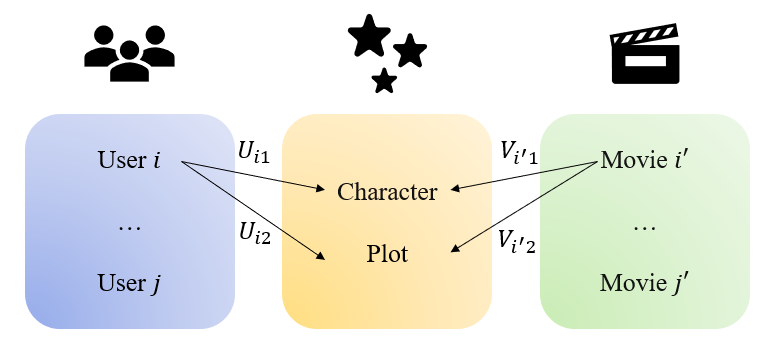
\includegraphics[scale=0.4]{pic/figure1.png}
  \caption{A Matrix Factorization Example with Dimension of Latent Features $=2$}
\end{figure} 

This model introduces a user-matrix $U_{m \times d}$ and an item-matrix $V_{n \times d}$, with 
$U_{ij}$ being the attention user $i$ pays in feature $j$, and $V_{kj}$ be the score of item $k$ 
earns in feature $j$. It predicts the rating matrix $R_{m \times n}$ (i.e. $R_{ij}: $ the rating of user $i$ on item $j$) 
by $R \approx U V^T$. The model can be trained by minimizing the distance
$$ \min_{U, V} \mathcal{L} = \frac{1}{2} \Vert R - UV^T \Vert_F^2 $$
Here $\Vert \cdot \Vert_F$ denotes the Frobenius norm. 
By adding regularization, due to the sparsity of $R$, it is often rewritten as
\begin{equation}
  \min_{U, V} \mathcal{L} = \frac{1}{2} \{\sum_{i=1}^m \sum_{j=1}^n I_{ij} (R_{ij} - U_iV_j^T)^2 + \lambda_1 \Vert U \Vert_F^2 + \lambda_2 \Vert V \Vert_F^2 \}
\end{equation} 
where $m$ is the number of users, $n$ is the number of items, $\mathcal{N}(i)$ is 
the neighbours of user i, $I_{ij} \in \{0, 1\}$ indicates whether user $i$ has rated item $j$. 
Many social recommending approaches \cite{ma2011rsr, jam2010trust, ma2009rste} are based on this framework.
\subsection{Social Regularization}
SR improves MF by utilizing information in social network. Fig 2. shows an exmaple in real world rating website. The key idea is that a movie 
received many positive feedbacks among your friends will more probably attract you. 
Therefore it is rational that the user in Fig 2. gives "Star Wars" a high score. 

\begin{figure}[h]
  \centering
  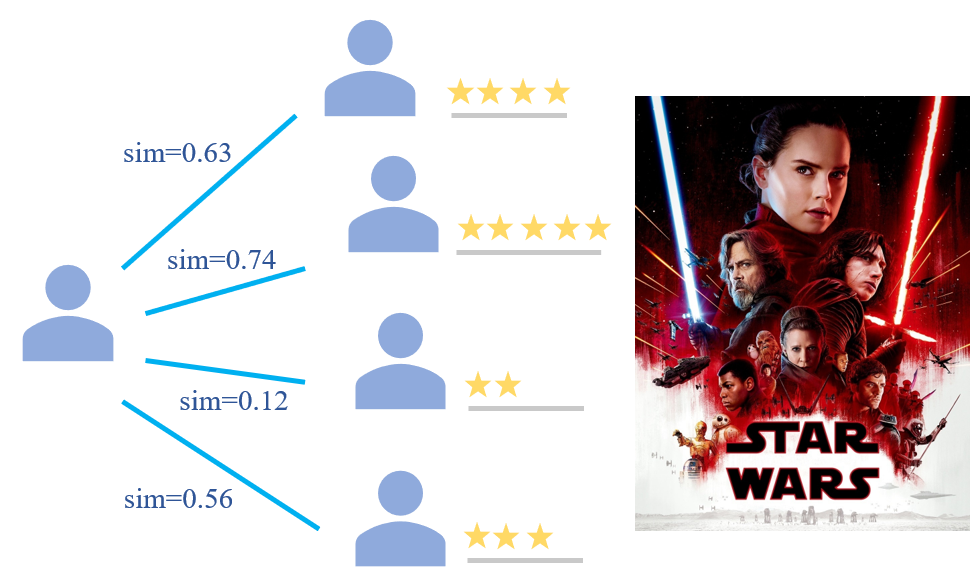
\includegraphics[scale=0.35]{pic/figure2.png}
  \caption{A Social Network Constraint Example}
\end{figure}

However, the friendship does not always bring consensus, which inspires us to introduce 
a similarity to weigh our friends. The most widely used method is 
Pearson Correlation Coefficient (PCC) \cite{bre1998pcc}.

\begin{equation}
  {Sim}(u, v) = \frac{\sum_{I_{ui} I_{vi} = 1} (R_{ui} - \overline{R_u}) (R_{vi} - \overline{R_v}) }
  {\sqrt{\sum_{I_{ui} I_{vi} = 1} (R_{ui} - \overline{R_u})^2} \cdot \sqrt{\sum_{I_{ui} I_{vi} = 1} (R_{vi} - \overline{R_v})^2}}
\end{equation}

And the model is proposed by minimizing the loss
\begin{equation}
  \min_{U, V} \mathcal{L} = \frac{1}{2} \{\sum_{i=1}^m [\sum_{j=1}^n I_{ij} (R_{ij} - U_iV_j^T)^2 + \beta \sum_{v \in \mathcal{N}(i)} {Sim}(i, v) \Vert U_i - U_v \Vert_F^2 ] + \lambda_1 \Vert U \Vert_F^2 + \lambda_2 \Vert V \Vert_F^2 \}
\end{equation}
\section{Method}
\label{method}
Still there are some limitations in SR as it weighs friends only by similarity. 
We improves SR by further analyzing the network and adding two dimensions: influence and familiarity. To be specific, 
our TriSR uses $Tri(i, u)$ to weigh the relationship between $i$ and $u$ which is defined as \\
\begin{equation}
  Tri(i, u) = \sqrt{(\alpha {Inf}(u))^2 + (\beta {Sim}(i, u))^2 + (\gamma {Fam}(i, u))^2 }
\end{equation}

where ${Inf}(u)$ is the influence of $u$ and $Fam(i, u)$ is the familiarity between $i$ and $u$. 
\begin{figure}[h]    
  \centering
  \begin{subfigure}{0.26\textwidth}
    \centering
      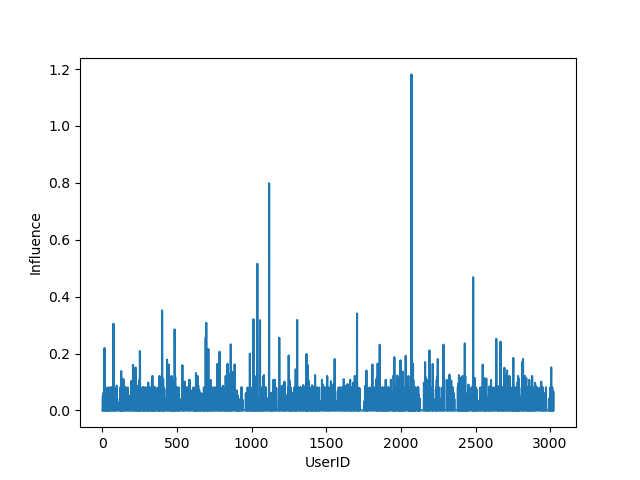
\includegraphics[width=1\linewidth]{pic/figure3_1.png}
  \end{subfigure}%
  \begin{subfigure}{0.26\textwidth}
  \centering
      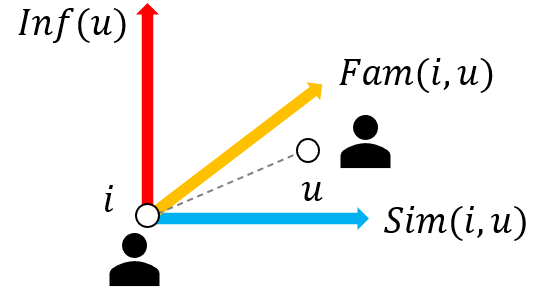
\includegraphics[width=1\linewidth]{pic/figure3_2.png}
  \end{subfigure}%
\caption{Comparsion between $Sim(i,u)$ (1 dimension) and $Tri(i,u)$ (3 dimensions)}
\end{figure}
\subsection{Influence Analysis}

The influence in a network obeys the Power Law Distribution, 
meaning only a small group of people are the celebrities of this network.
Usually a recommendation from a big movie blogger is more convincible than a casual user, 
which inspires us to adjust our model by influence.

Influence Analysis is a traditional topic and there are many recent approaches like VoteRank \cite{zhang2016voterank}.
But we choose the classical PageRank \cite{ser1998pagerank} due to its high effectiveness in online situation. 
The influence can be analyzed iteratively through a Markov Process.
\begin{equation}
   Inf^t(i) = p \sum_{v \in \mathcal{N}(i)} \frac{Inf^{t-1}(v)}{\deg(v)} + (1-p) \cdot \frac{1}{m}
\end{equation}
where $p$ is a hyperparameter usually set to $0.85$. 
Fig 4. illustrates the distribution of the influence in our datasets 
which factually obeys power law distribution.
\begin{figure}[h]    
    \centering
    \begin{subfigure}{0.33\textwidth}
      \centering
        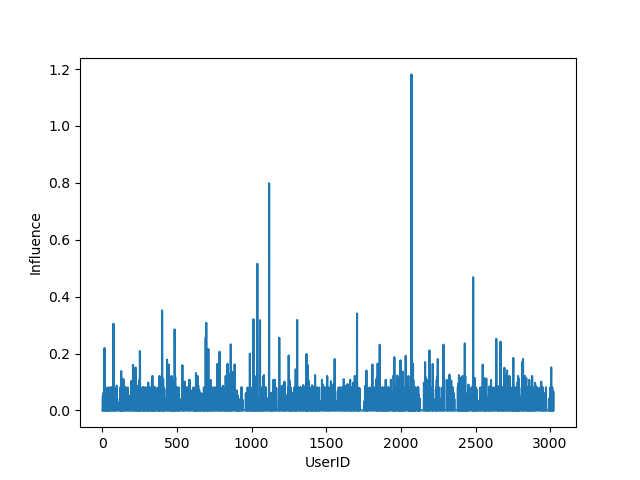
\includegraphics[width=1\linewidth]{pic/figure4_1.png}
      \caption{Douban}
    \end{subfigure}%
    \begin{subfigure}{0.33\textwidth}
    \centering
        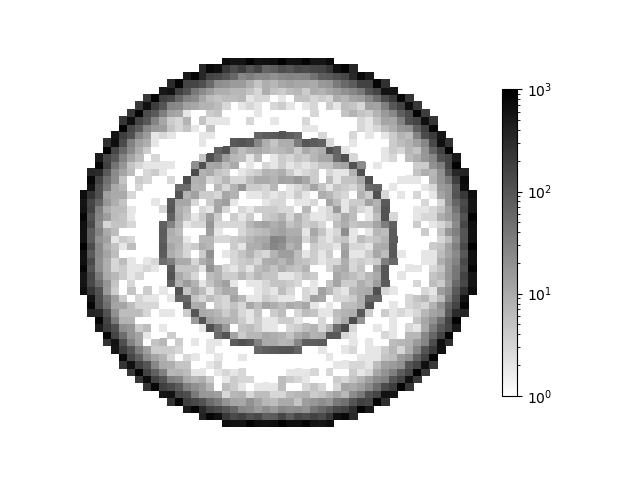
\includegraphics[width=1\linewidth]{pic/figure4_2.png}
      \caption{Dianping}
    \end{subfigure}%
    \begin{subfigure}{0.33\textwidth}
      \centering
        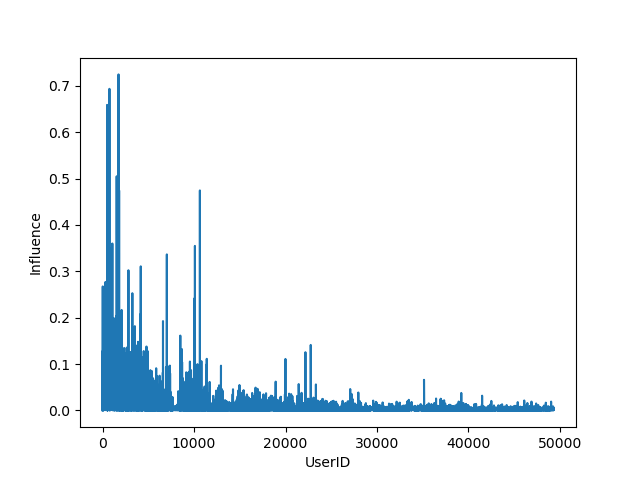
\includegraphics[width=1\linewidth]{pic/figure4_3.png}
        \caption{Epinions}
    \end{subfigure}
  \caption{The Distribution of Influence}
\end{figure}
\subsection{Familiarity}
Another noteworthy weight is the familiarity between users in real world
because familiars not only have a greater chance to recommend but a higher credibility 
based on the idea that "familiars will not cheat us". 

We adopt a direct familiarity measure \cite{liang2012pr} according to the proportion of common friends.
\begin{equation}
  {Fam}(u, v) = \frac{|\mathcal{N}(u) \cap \mathcal{N}(v)|}{\sqrt{|\mathcal{N}(u)|} \sqrt{|\mathcal{N}(v)|}}
\end{equation}
\subsection{Our Model}
By combining (2), (4), (5) and (6), the objective function of TriSR can be formulated as
\begin{equation}
  \min_{U, V} \mathcal{L} = \frac{1}{2} \{\sum_{i=1}^m [\sum_{j=1}^n I_{ij} (R_{ij} - U_iV_j^T)^2 + \sum_{v \in \mathcal{N}(i)} Tri(i, v) \Vert U_i - U_v \Vert_F^2 ] + \lambda_1 \Vert U \Vert_F^2 + \lambda_2 \Vert V \Vert_F^2 \}
\end{equation}
with three hyperparameters $\alpha$, $\beta$, $\gamma$ indicates the importance of each dimension in $Tri$. 
To visualize the difference between similarly and $Tri$, we choose the user with the most friends in Dianping, drawing the distribution 
of the distance between him and his friends. Fig 5. shows that $Tri$ has a smoother distribution.
\begin{figure}[h]    
  \centering
  \begin{subfigure}{0.4\textwidth}
    \centering
      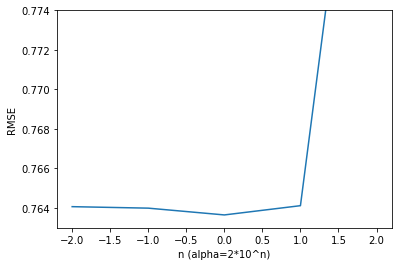
\includegraphics[width=1\linewidth]{pic/figure5_1.png}
    \caption{Similarity}
  \end{subfigure}%
  \begin{subfigure}{0.4\textwidth}
  \centering
      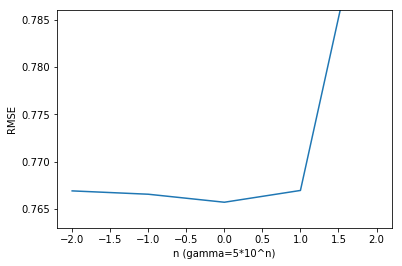
\includegraphics[width=1\linewidth]{pic/figure5_2.png}
    \caption{$Tri$}
  \end{subfigure}%
\caption{The Distribution of the Distance to the User with the Most Friends in Dianping}
\end{figure}
\section{Experiments}
\label{experiments}

\subsection{Datasets}
Our experiments are performed on three different datasets: Douban\footnote{https://www.douban.com} \cite{doubands}, 
Dianping \footnote{https://www.dianping.com} \cite{dianpingds} and Epinions \footnote{https://www.epinions.com} \cite{epinionsds}. Each dataset consists of two parts: historical ratings and a undirected social network.
All rating scores are scaled to $(0, 5]$.
\begin{table}[h]
  \caption{Statistics of Datasets}
  \label{sample-table}
  \centering
  \begin{tabular}{llll}
    \toprule
    Dataset  & Douban  & Dianping & Epinions \\
    \midrule
    Users & 3022     & 147918     & 49289  \\
    Items & 6977     & 11123      & 139738 \\
    Ratings & 195493 & 2149675    & 664824 \\
    Social Relationships & 1366 & 629618 & 487181 \\
    \bottomrule
  \end{tabular}
\end{table}
\subsection{Metrics and Competitors}
We mainly use two popular metrics in the field of recommender systems: 
Mean Absolute Error (MAE) and Root Mean Square Error (RMSE). They are defined as follows.
$$
MAE = \frac{\sum_{(i, j, R_{ij}) \in T} |\hat{R}_{ij} - R_{ij}|}{|T|}
$$
$$
RMSE = \sqrt{ \frac{\sum_{(i, j, R_{ij}) \in T} (\hat{R}_{ij} - R_{ij})^2}{|T|} }
$$
where $T$ is the test set with each test rating being a triple $(user, item, score)$.

We evaluate the performance in our self-implemented benchmark (see the code attached). 
To provide a conprehensive view, we adopt the following methods as competitors.
\begin{itemize}
  \item \textbf{UserMean} predicts the rating $(user, item, score)$ by the average rating scores of $user$.
  \item \textbf{ItemMean} predicts the rating $(user, item, score)$ by the average rated scores of $item$.
  \item \textbf{UserCF} is a Collaborative Filtering algorithm focusing on users. 
  It predicts the rating $(user, item, score)$ by the average rating scores of 
  Top-N most similar users of $user$.
  \item \textbf{ItemCF} \cite{Sarwar2001ItembasedCF} is the same with UserCF but it focuses on items.
  \item \textbf{MF} is the matrix factorization method.
  \item \textbf{SR} is a matrix factorization with social regularization based on similarity.
  \item \textbf{TriSR} improves SR with a more detailed three-dimensional social regularization.
\end{itemize}
After performing 5-fold cross-validation, the parameters are set as follows: 
On Douban and Dianping, $\lambda_1 = \lambda_2 = 0.01$ for all methods. $\beta = 5$ for SR and 
$\alpha=2, \beta=5, \gamma=3$ for TriSR. On Epinions, $\lambda_1 = \lambda_2 = 10^{-5}$, $\beta=0.55$ 
and $\alpha=0.25, \beta=0.5, \gamma=0.25$. For the dimension of latent 
features $d$, we adopt $d=10$ on Douban and $d=20$ on Dianping and Epinions. 

We test each model 5 times in the benchmark and take the average as the result. 
On Douban and Dianping, we take $60\%$ data for training and the rest for testing while 
the rate is $90\%$ in Epinions. We use Adam (at first) and Mini-batch SGD (close to convergence) to training.

\subsection{Results}

\begin{table}[h]
  \caption{Experiment Results}
  \centering
  \begin{tabular}{lllllllll}
    \toprule
    Dataset  & Metrics  & UserMean & ItemMean & UserCF & ItemCF & MF & SR & TriSR \\
    \midrule
    \midrule
    Douban   & MAE      &  0.6961  & 0.6265   & 0.6874 & 0.7462 & 0.5984  & 0.5973 & \textbf{0.5959} \\
             & RMSE     &  0.8675  & 0.7875   & 0.8743 & 0.9440 & 0.7625  & 0.7614 & \textbf{0.7597} \\
    \midrule
    Dianping & MAE      & 0.5314   & 0.5127   & 0.5351 & 0.5464 & 0.5048 & 0.5034 & \textbf{0.5033} \\
             & RMSE     & 0.7216   & 0.6702   & 0.7044 & 0.7835 & 0.6700 & \textbf{0.6674} & 0.6677 \\
    \midrule
    Epinions & MAE      & 0.9369   & 0.9421   & 0.9827 & 0.9873 & 0.9251 & 0.9183   & \textbf{0.9180} \\
             & RMSE     & 1.2072   & 1.2243   & 1.2942 & 1.3314 & 1.1920 & 1.1832   & \textbf{1.1824} \\
    \bottomrule
  \end{tabular}
\end{table}

\subsection{Impact of Parameters}
Since $\beta$ in our model is similar with $\beta$ in SR, here we 
only do some experiments in $\alpha$ and $\gamma$ on Douban dataset. 
As is shown in Fig 6. , a large parameter ($\sim 10^2$) 
leads to a catastrophe but a small one ($\sim 10^{-2}$) does not lose too much performance 
because it approximates to the SR model. 
And it also shows that $\alpha=2$, $\gamma=5$ ($\sim 10^{0}$) is relatively optimal.
\begin{figure}[h]    
  \centering
  \begin{subfigure}{0.4\textwidth}
    \centering
      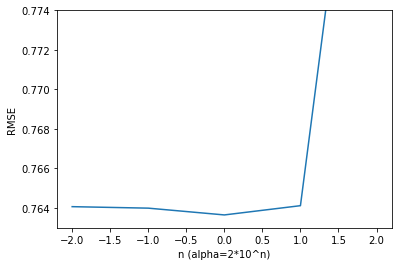
\includegraphics[width=1\linewidth]{pic/figure6_1.png}
    \caption{Impact of $\alpha$}
  \end{subfigure}%
  \begin{subfigure}{0.4\textwidth}
  \centering
      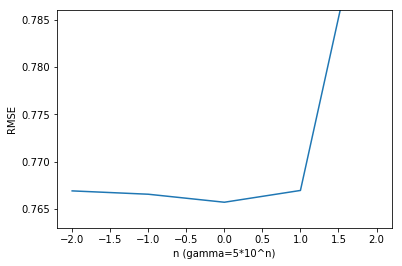
\includegraphics[width=1\linewidth]{pic/figure6_2.png}
    \caption{Impact of $\gamma$}
  \end{subfigure}%
\caption{Impact of Parameters}
\end{figure}
\section{Conclusion}
\label{conclusion}
The result shows that TriSR has a slightly better performance in most cases, except 
the RMSE metric in Dianping. A possible explanation might be that Dianping is a platform 
concentrating more on items, which also explains that ItemMean performs better in this test point. 

Based on this idea, we can classify different recommender systems into two categories: 
user-oriendted and item-oriented, by comparing the performance of UserMean and ItemMean.
TriSR has a better performance in a user-oriented platform like Douban and Epinions due to
our utilization of users' social information.

However, the improvement is not so much as we except. Further work on item-oriented 
platforms and directed social network is needed. 

\bibliographystyle{abbrv}
\bibliography{references}

\end{document}